\section{More on Processing}

\subsection{Primitives}
\begin{frame}[fragile]{Window Size}{}
    \Large
    \begin{minted}{c++}
        int width = 800;
        int height = 400;
    \end{minted}
    \pause
    \begin{minted}{c++}
        size(width, height);
    \end{minted}
    \pause
    \begin{minted}{c++}
        // The wrong way to specify
        // the middle of the screen
        ellipse(400, 200, 50, 50);
    \end{minted}
    \pause
    \begin{minted}{c++}
        // Always the middle
        // no matter how size() changes
        ellipse(width/2, height/2, 50, 50);
    \end{minted}
\end{frame}

\begin{frame}[fragile]{Rectangle}{}
    \Large
    \begin{minted}{c++}
        rect(a, b, c, d);
        rect(a, b, c, d, r);
        rect(a, b, c, d, tl, tr, br, bl);
    \end{minted}
    \pause
    \begin{minted}{text}
    a   float: x-coordinate of rectangle
    b   float: y-coordinate of rectangle
    c   float: width of the rectangle
    d   float: height of the rectangle
    \end{minted}
    \pause
    \begin{minted}{text}
    r   float: radii for all four corners
    \end{minted}
    \pause
    \begin{minted}{text}
    tl  float: radius of top-left corner
    tr  float: radius of top-right corner
    br  float: radius of bottom-right corner
    bl  float: radius of bottom-left corner
    \end{minted}
\end{frame}

\begin{frame}[fragile]{rect() Examples}{}
\begin{figure}
    \begin{center}
        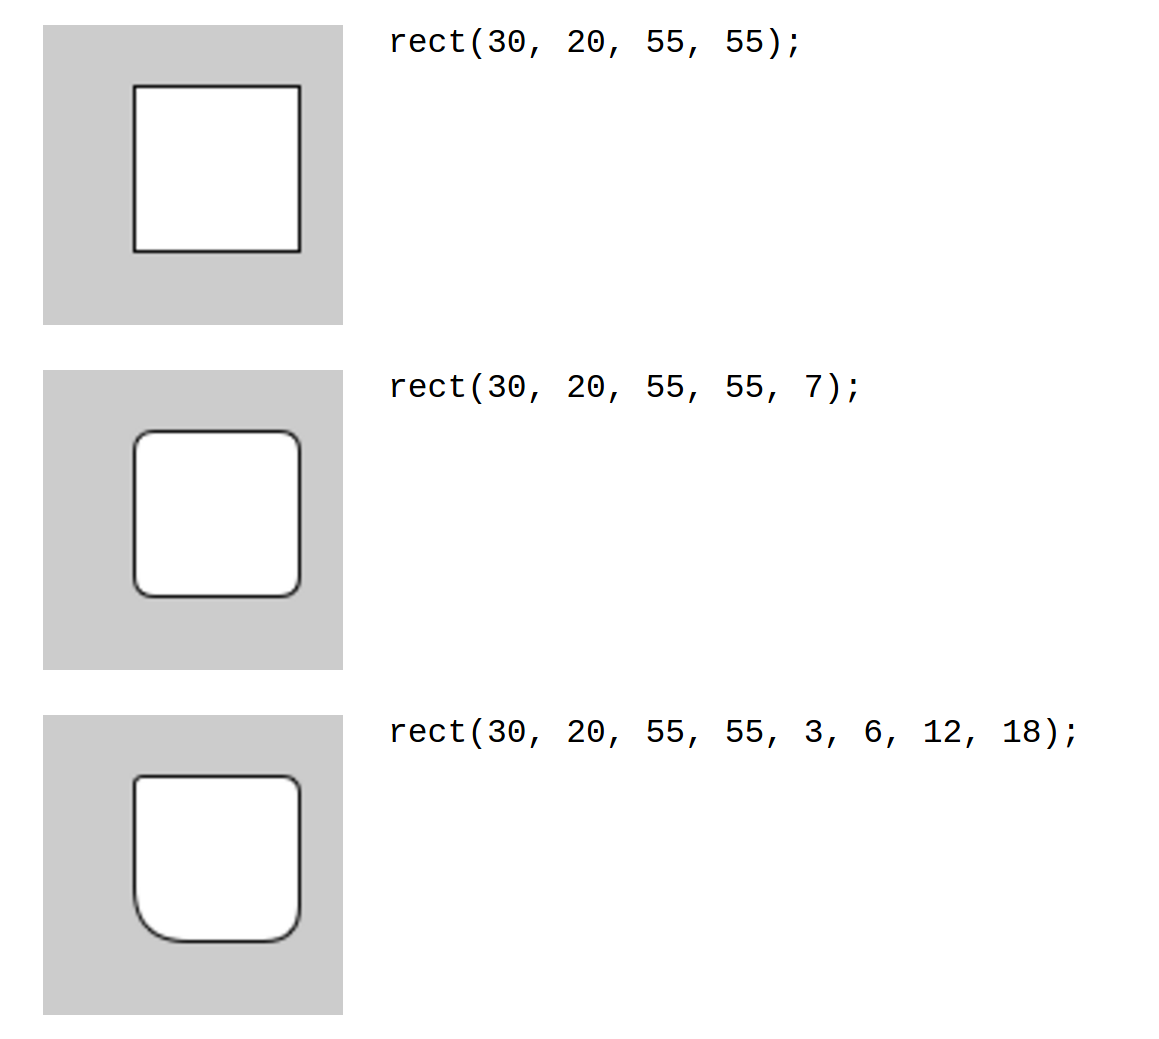
\includegraphics[width=.7\linewidth]{images/rect.png}
    \end{center}
\end{figure}
\end{frame}

\subsection{Coordinate System}
\begin{frame}[fragile]{Normal Coordinate System}{}
\begin{figure}
    \begin{center}
        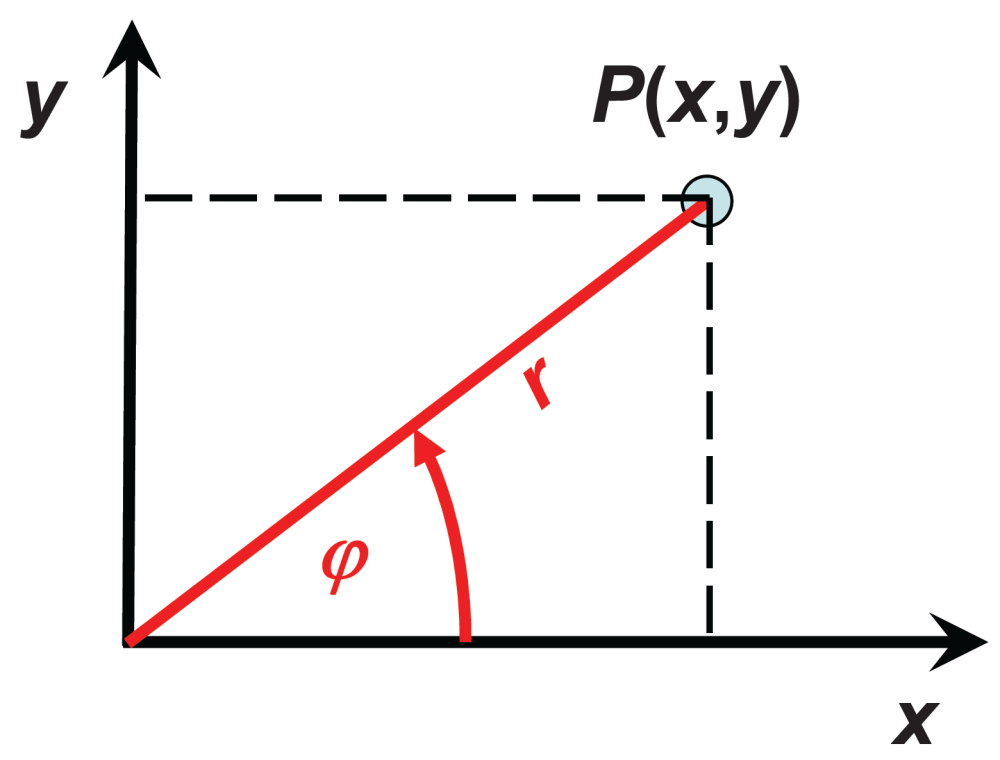
\includegraphics[width=.8\linewidth]{images/normal_coord.png}
    \end{center}
\end{figure}
\end{frame}

\begin{frame}[fragile]{Processing Coordinate System}{}
\begin{figure}
    \begin{center}
        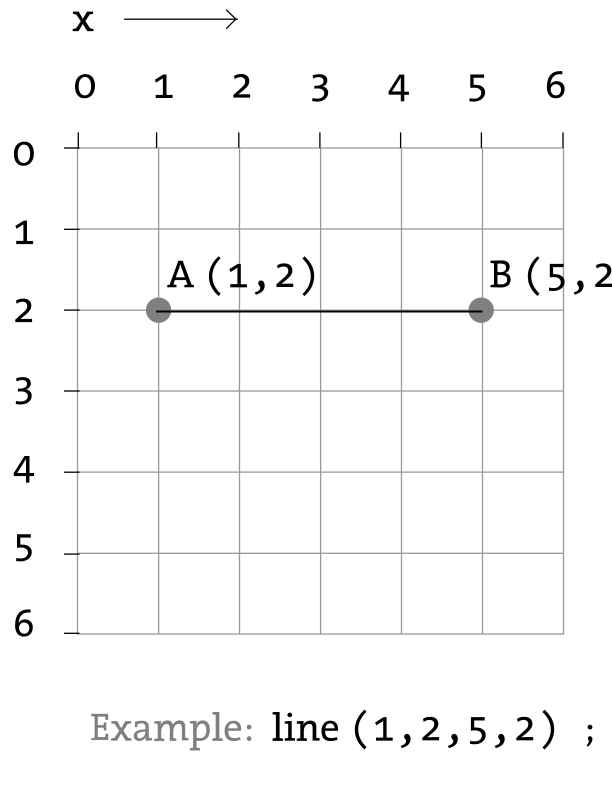
\includegraphics[width=.6\linewidth]{images/processing_coord.png}
    \end{center}
\end{figure}
\end{frame}

\begin{frame}[fragile]{Drawing a Rectangle}{}
\begin{figure}
    \begin{center}
        \def\svgwidth{\columnwidth}
        \input{images/rect_normal.pdf_tex}
    \end{center}
\end{figure}
\end{frame}

\begin{frame}[fragile]{CENTER Rectangle}{}
\begin{figure}
    \begin{center}
        \def\svgwidth{0.9\columnwidth}
        \input{images/rect_center.pdf_tex}
    \end{center}
\end{figure}
\end{frame}

\begin{frame}[fragile]{CORNERS Rectangle}{}
\begin{figure}
    \begin{center}
        \def\svgwidth{0.9\columnwidth}
        \input{images/rect_corners.pdf_tex}
    \end{center}
\end{figure}
\end{frame}


\subsection{Debugging}
\begin{frame}[fragile]{Print Statements}{}
    \begin{itemize}
    \item print() statement prints all items separated by spaces
    \begin{minted}{cpp}
    print(item1, item2, . . . );
    \end{minted}
    \pause
    \item println() is the same, but prints a new line at the end
    \begin{minted}{cpp}
    println(item1, item2, . . . );
    \end{minted}
    \end{itemize}
\end{frame}


\subsection{Interaction}
\begin{frame}[fragile]{Mouse Handling}{}
    \begin{itemize}
    \item Mouse position -- Global Variables
    \begin{minted}{cpp}
    mouseX, mouseY
    ellipse(mouseX, mouseY, 2*R, 2*R);
    \end{minted}
    \pause
    \item Detect Mouse Click
    \begin{minted}{cpp}
    if (mousePressed) {
       fill(255); // White
    } else {
        fill(0); // Black
    }
    \end{minted}
    \end{itemize}
\end{frame}

\begin{frame}[fragile]{Keyboard Handling}{}
    \Large
    \begin{minted}{cpp}
    char LEFT = 'a', RIGHT = 'd', UP = 'w';
    boolean left, right, up;
    \end{minted}
    \pause
    \begin{minted}{cpp}
    void keyPressed() {
        if (key == LEFT)       left = true;
        if (key == RIGHT)      right = true;
        if (key == UP)         up = true;
    }
    \end{minted}
    \pause
    \begin{minted}{cpp}
    void keyReleased() {
        if (key == LEFT)       left = false;
        if (key == RIGHT)      right = false;
        if (key == UP)         up = false;
    }
    \end{minted}
\end{frame}

\begin{frame}[fragile]{Keyboard Handling}{}
    \huge
    \begin{minted}{cpp}
    if (left) {
        // Move Left . . .
    }
    if (right) {
        // Move Right . . .
    }
    if (up) {
        // Move Up . . .
    }
    \end{minted}
\end{frame}

\subsection{Physics}
\begin{frame}[fragile]{Define Position and Velocity}{}
    \Large
    \begin{minted}{cpp}
    float ballX = width/2, ballY = height/2;
    float ballVx = 2, ballVy = 3;
    \end{minted}
    \pause
    \begin{minted}{cpp}
    void draw() {
        ellipse(ballX, ballY, 2*R, 2*R);
        updateBallPosition();
    }
    \end{minted}
    \pause
    \begin{minted}{cpp}
    void updateBallPosition() {
        ballX += ballVx;
        ballY += ballVy;
    }
    \end{minted}
\end{frame}

\begin{frame}[fragile]{Gravity}{}
    \Large
    \begin{minted}{cpp}
    float gravity = 1;
    \end{minted}
    \pause
    \begin{minted}{cpp}
    void draw() {
        ellipse(ballX, ballY, 2*R, 2*R);
        updateBallVelocity();
        updateBallPosition();
    }
    \end{minted}
    \pause
    \begin{minted}{cpp}
    void updateBallVelocity() {
        ballVy += gravity;
    }
    \end{minted}
\end{frame}


\subsection{Exercise}
\begin{frame}[fragile]{Forking}{}
    \begin{block}{}
        Go to https://github.com/amartyashankha/MIRP2017\_movement
    \end{block}
    \begin{block}{Click on Fork}
        \begin{figure}
            \begin{center}
                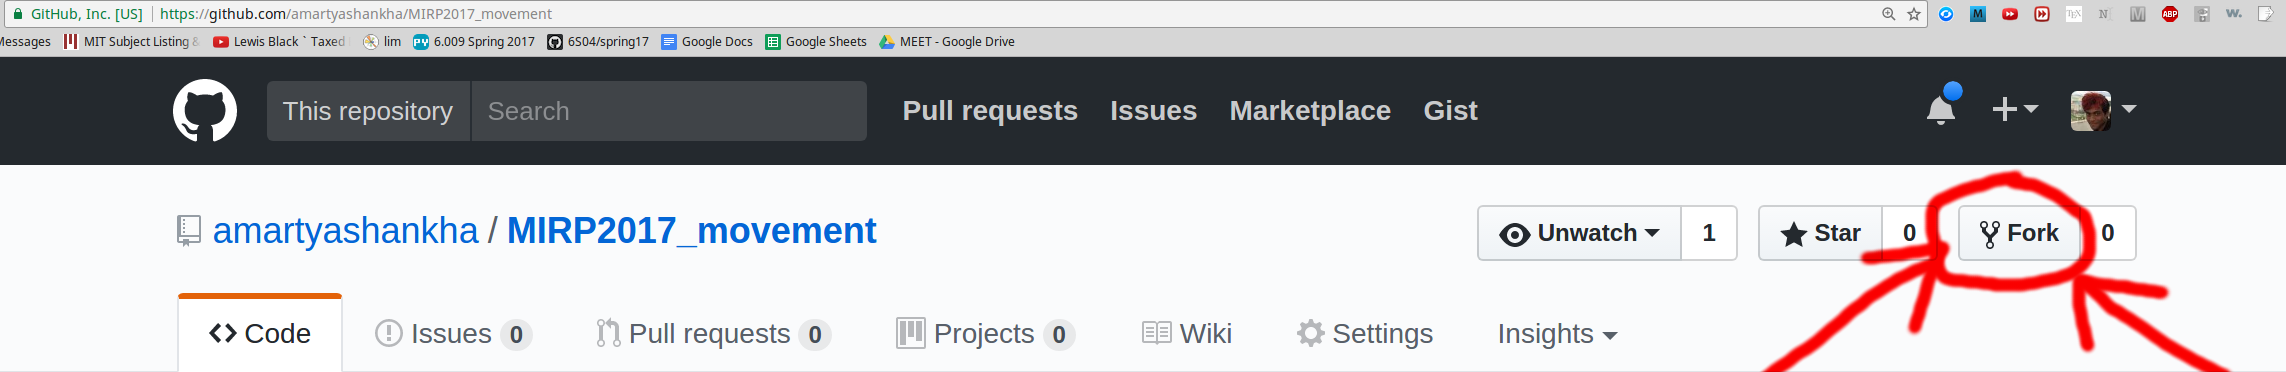
\includegraphics[width=\linewidth]{images/git_fork.png}
            \end{center}
        \end{figure}
    \end{block}
    \begin{block}{The title should change}
        \begin{figure}
            \begin{center}
                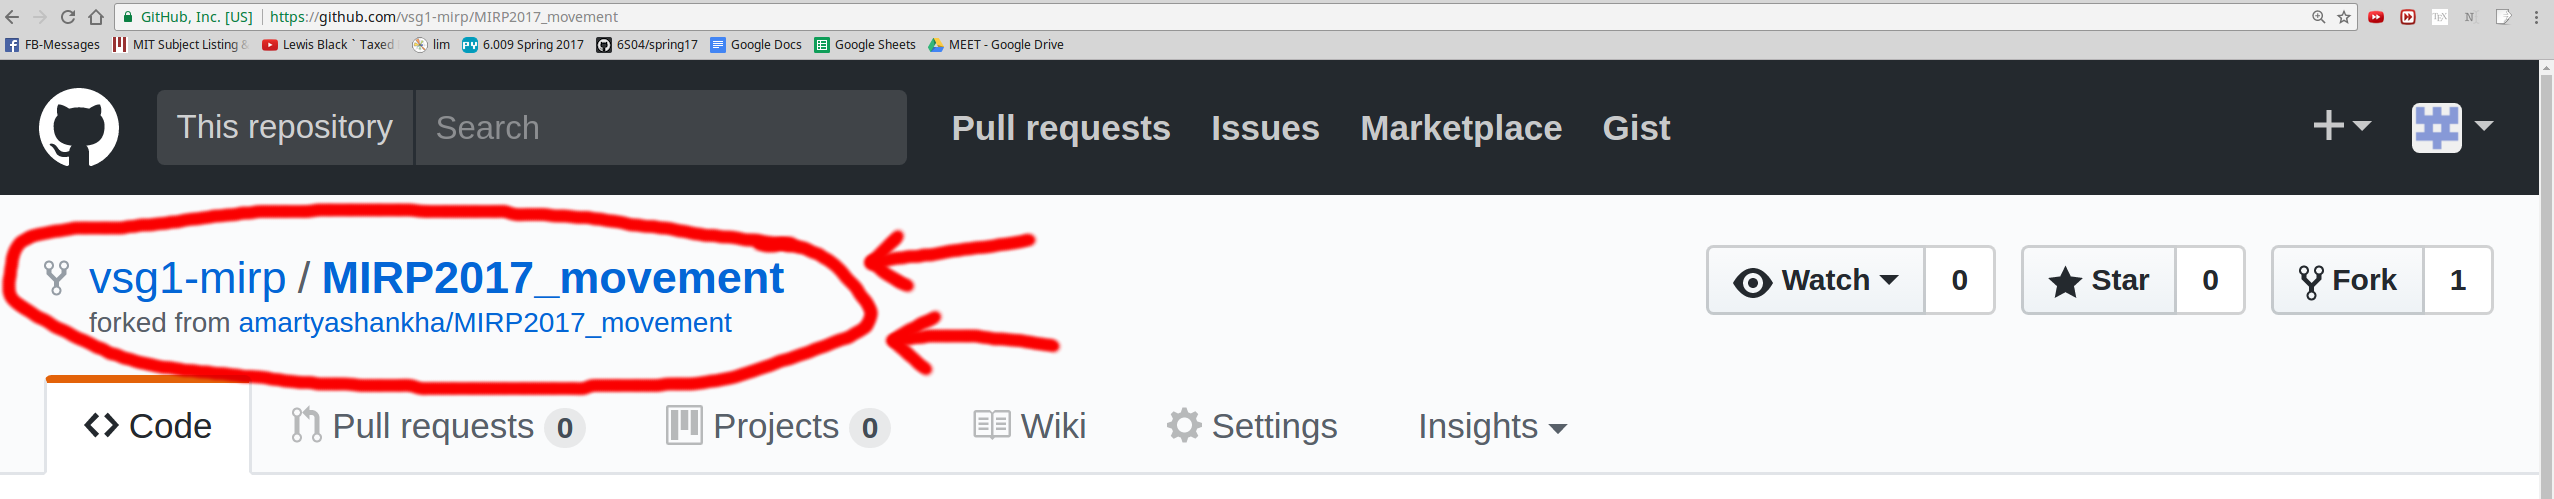
\includegraphics[width=\linewidth]{images/git_forked.png}
            \end{center}
        \end{figure}
    \end{block}
\end{frame}

\begin{frame}[fragile]{Cloning}{}
    \begin{block}{Clone the repo}
        \begin{figure}
            \begin{center}
                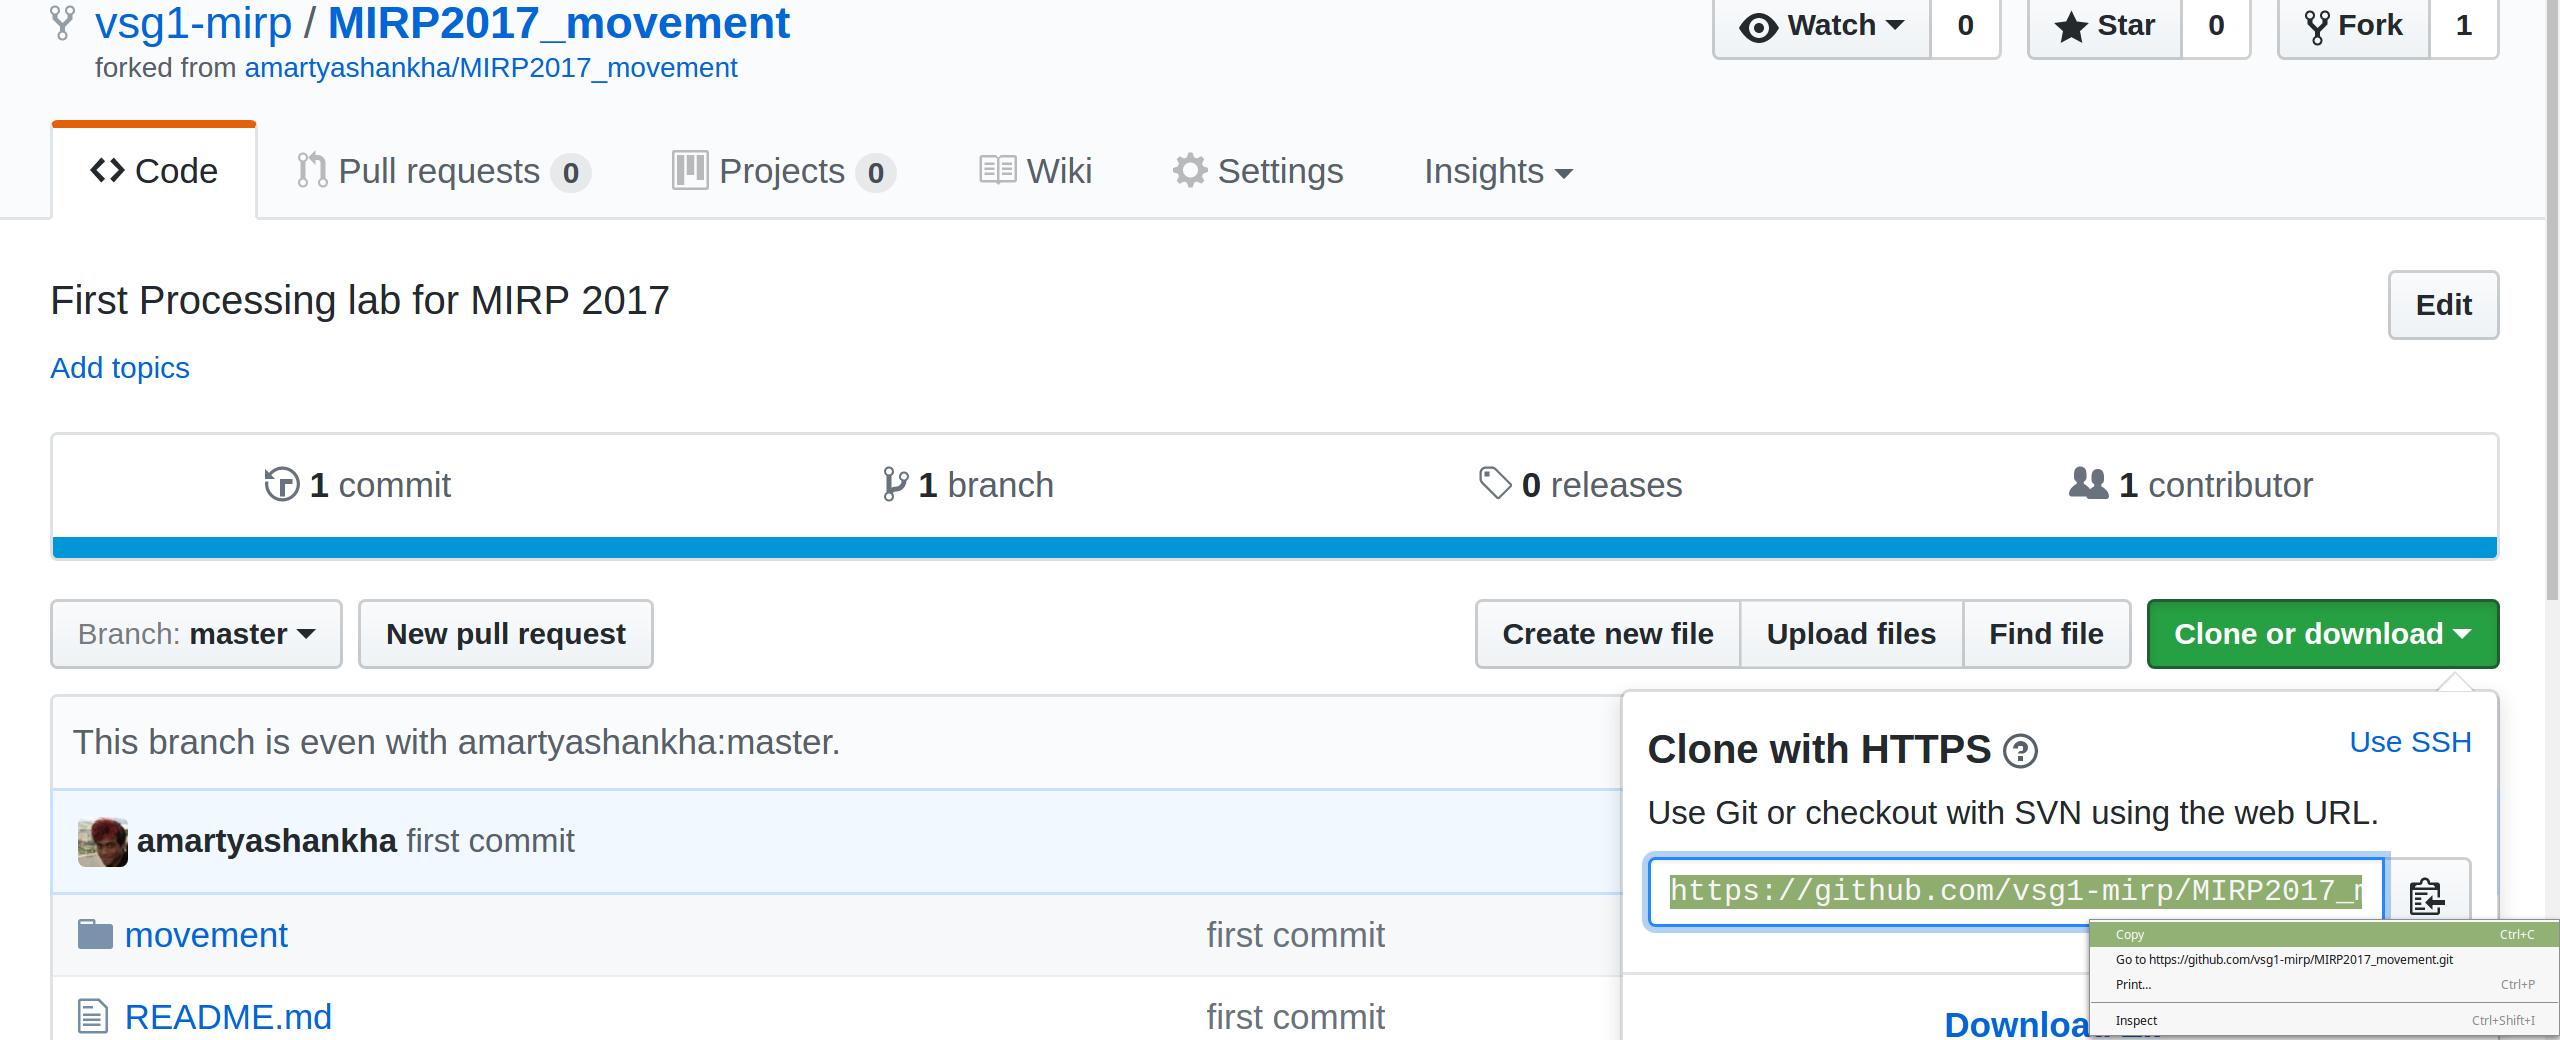
\includegraphics[width=0.8\linewidth]{images/git_clone.png}
            \end{center}
        \end{figure}
    \end{block}
    \begin{itemize}
        \item Open Processing
        \item File $\rightarrow$ Open
        \item Navigate to the files inside Movement 
    \end{itemize}
\end{frame}

\begin{frame}[fragile]{Exercise}{}
    \LARGE
    \begin{block}{}
    Resolve collisions with other walls.
    Move ball using WASD.
    \end{block}
    \begin{block}{}
    Move ball using WASD.
    \end{block}
\end{frame}
